\chapter{Special Unitary Group $\mathrm{SU}(3, \, \C)$} \thispagestyle{empty}
\label{chwk}

In this chapter, we study more in-depth the special unitary (Lie) group $\mathrm{SU}(3, \, \C)$ and the associated Lie algebra $\mathrm{su}(3, \, \C)$. Recall that the set of all unitary matrices
\begin{equation*} \mathrm{U}(N, \, \C) := \left\{ U \in \mathrm{GL}(N, \, \C) \: : \: U^\dag U = U U^\dag = \mathrm{Id}_{N \times N} \right\} \end{equation*}
is a group with respect to the matrix product. Similarly,
\begin{equation*} \mathrm{SU}(N, \, \C) := \left\{ U \in \mathrm{GL}(N, \, \C) \: : \: U^\dag U = U U^\dag = \mathrm{Id}_{N \times N}, \: \mathrm{det}(U) = 1 \right\} \end{equation*}
is also a group, and it is called \textit{special unitary group}.

The eight generators of the $3$-special unitary group can be computed explicitly in the fundamental representation (=smallest nontrivial), and they are given by the \textit{Gell-Mann matrices}\index{Gell-Mann matrices}:
\begin{equation*}\begin{aligned} & \lambda^1 = \frac{1}{2} \begin{pmatrix} 0 & 1 & 0 \\ 1 & 0 & 0 \\ 0 & 0 & 0 \end{pmatrix}, \qquad \lambda^2 = \frac{1}{2} \begin{pmatrix} 0 & - \imath & 0 \\ \imath & 0 &0 \\ 0 & 0 & 0 \end{pmatrix}, \qquad \lambda^3 = \frac{1}{2} \begin{pmatrix} 1 & 0 &0 \\ 0 & - 1 & 0 \\ 0 & 0 & 0\end{pmatrix},
\\[1em] & \lambda^4 = \frac{1}{2} \begin{pmatrix} 0 & 0 & 1 \\ 0 & 0 & 0 \\ 1 & 0 & 0 \end{pmatrix}, \qquad \lambda^5 = \frac{1}{2} \begin{pmatrix} 0 & 0 & - \imath \\ 0 & 0 & 0 \\ \imath & 0 & 0 \end{pmatrix}, \qquad \lambda^6 = \frac{1}{2} \begin{pmatrix} 0 & 0 & 0 \\ 0 & 0 & 1 \\ 0 & 1 & 0 \end{pmatrix},
\\[1em] & \lambda^7 = \frac{1}{2} \begin{pmatrix} 0 & 0 & 0 \\ 0 & 0 & -\imath \\ 0 & \imath & 0 \end{pmatrix}, \qquad \lambda^8 = \frac{1}{2\sqrt{3}} \begin{pmatrix} 1 & 0 & 0 \\ 0 & 1 & 0\\ 0 & 0 & -2  \end{pmatrix} .\end{aligned} \end{equation*}
We immediately see that $\mathrm{SU}(2, \, \C)$ is generated by $\lambda^1$, $\lambda^2$ and $\lambda^3$, and it is thus a subgroup of $\mathrm{SU}(3, \, \C)$. Moreover, one can easily prove that
\begin{equation*}\mathrm{tr}(\lambda^a \lambda^b) = \frac{1}{2} \delta_{ab} \quad \text{and} \quad f^{abc} = \begin{cases} 1 & \text{if $(a b c) = (1 2 3)$,} \\[0.5em] 1/2 & \text{if $(a b c) \in \{(345), \, (147), \, (246), \, (257) \}$ ,} \\[0.5em] - 1/2 & \text{if $(abc) \in \{(156), \, (367)\}$,} \\[0.5em] \sqrt{3}/2 & \text{if $(abc) \in \{ (458), \, (678) \}$}, \end{cases}\end{equation*}
which determines all the possible values of $f^{abc}$ since it is a completely antisymmetric tensor.

\paragraph{Killing Form.} We can easily check that the killing form \eqref{kf} is given by
\begin{equation*} g^{ab} := f^{acd} f^{bdc} = - \frac{3}{2} \delta_{ab} \quad \text{for all $a, \, b = 1, \, \dots, \, 8$}. \end{equation*}
Recall that a \textit{Casimir Operator} is a precise element which lies within the center of a Lie algebra (e.g., the square of the angular momentum modulus in $\mathrm{so}(3, \, \R)$).

Let $\g$ be a \textbf{semisimple} Lie algebra, and let $g^{ab}$ denote its metric \eqref{kf}. The matrix $g$ is invertible by Cartan's criterion, and therefore we can introduce the following notation:
\begin{equation*} g_{ab} := (g^{-1})_{ab} \end{equation*}
The (quadratic) \textit{Casimir operator} of the semisimple Lie algebra $\mathrm{su}(3, \, \C)$ is defined by setting
\begin{equation} \label{caso1} C := g_{ab}\lambda^a\lambda^b. \end{equation}

\begin{lemma} The Casimir operator $C$ is an element of the center $C(\g)$, that is,
\begin{equation*} [C, \, T^a] = 0 \quad \text{for every $T^a \in \g$}. \end{equation*} \end{lemma}

Recall also that, if we define $c_{abc} := g^{ae} f^{bce}$, then it turns out that $c_{abc} = c_{bca} = c_{cab}$ and $c$ is totally antisymmetric. In particular, in the case of the special unitary group we have that
\begin{equation*} c_{abc} := - \frac{3}{2} f^{bca} \implies \text{$f^{bca}$ is also totally antisymmetric}.\end{equation*}

\section{Finite Irreducible Representations}

The primary goal is to find all the irreducible representations of $\mathrm{SU}(3, \, \C)$ and $\mathrm{su}(3, \, \C)$, starting here with the finite-dimensional\footnote{A representation\index{representation!finite-dimensional} is finite dimensional if and only if the carrying vector space $V$ has finite dimension.} ones.

\subsection{Construction via Weight Diagrams}

Let us consider the fundamental ($3$-dimensional) representation
\begin{equation*} \underline{3} \: : \: \begin{pmatrix} q_1 \\ q_2 \\ q_3 \end{pmatrix} \quad \text{where $| \, q_1 \rangle = \begin{pmatrix} 1 \\ 0 \\ 0 \end{pmatrix}$, $|\, q_2 \rangle = \begin{pmatrix} 0 \\ 1 \\ 0 \end{pmatrix}$ and $|\,q_3 \rangle = \begin{pmatrix} 0 \\ 0 \\ 1 \end{pmatrix}$.} \end{equation*}
The generators $\lambda^3$ and $\lambda^8$ are both diagonal, and thus $\{ |\,q_i \rangle \: : \: i \in \{1, \, 2, \, 3\}\}$ is a basis for the both of them. Precisely, we have that
\begin{equation*} \begin{aligned} & \lambda^3 \,|\, q_1 \rangle = \frac{1}{2} \,|\, q_1 \rangle & \text{and} \qquad \lambda^8 \,|\,q_1 \rangle = \frac{1}{2 \sqrt{3}} \,|\,q_1 \rangle,
\\[1em] & \lambda^3 \,|\, q_2 \rangle = - \frac{1}{2} \,|\,q_2 \rangle & \text{and} \qquad \lambda^8 \,|\,q_2 \rangle = \frac{1}{2 \sqrt{3}} \,|\,q_2 \rangle,
\\[1em] & \lambda^3 \,|\,q_3 \rangle = 0 \,|\,q_3 \rangle & \text{and} \qquad \lambda^8 \,|\,q_3 \rangle = - \frac{1} {\sqrt{3}} \,|\,q_3 \rangle. \end{aligned} \end{equation*}
The vectors $q_i$ are $2$-dimensional vectors\footnote{The rank\index{group rank} of a group $\G$ is defined as the number of diagonal generators in the fundamental representation.} in the space generated by $\lambda^3$ and $\lambda^8$, whose coordinate are given by the relations above:
\begin{equation*} q_1 = \begin{pmatrix} \frac{1}{2} & \frac{1}{2 \sqrt{3}} \end{pmatrix}, \qquad q_2 = \begin{pmatrix} - \frac{1}{2} & \frac{1}{2 \sqrt{3}} \end{pmatrix}, \qquad q_3 = \begin{pmatrix} 0 & - \frac{1}{\sqrt{3}} \end{pmatrix}. \end{equation*}
If we consider the hypercharge operator\index{hypercharge operator} $Y := \frac{2}{\sqrt{3}} \lambda^8$, then the points $q_i$ delimits a regular triangle as in the figure below:
\begin{figure}[!htbp]
        \centering
        \mbox{%
\begin{minipage}{.40\textwidth}
\begin{tikzpicture}
\draw[help lines, color=gray!30, dashed] (-2.3,-2.3) grid (2.3,2.3);
\draw[->,ultra thin] (-2.4,0)--(2.4,0) node[right]{$\lambda^3$};
\draw[->,ultra thin] (0,-2.4)--(0,2.4) node[above]{$Y$};
  [anchor=mid west,
  mark size=+2pt, mark color=red,  ball color=green]
  \foreach \plm[count=\cnt] in {ball}
    \draw[mark options={fill=red}]
      plot[mark=\plm] coordinates {(1, 2/3) (-1, 2/3) (0, -4/3) (1, 2/3)};
	\node[] at (-1, 2/3+0.3) {$q_2$}; \node[] at (1, 2/3 + 0.3) {$q_1$}; \node[] at (0.3, -4/3) {$q_3$}; 
\end{tikzpicture}
          \end{minipage}%
          \qquad
          \begin{minipage}{.40\textwidth}
      \begin{tikzpicture}
\draw[help lines, color=gray!30, dashed] (-2.3,-2.3) grid (2.3,2.3);
\draw[->,ultra thin] (-2.4,0)--(2.4,0) node[right]{$\lambda^3$};
\draw[->,ultra thin] (0,-2.4)--(0,2.4) node[above]{$Y$};
  [anchor=mid west,
  mark size=+2pt, mark color=red,  ball color=green]
  \foreach \plm[count=\cnt] in {ball}
    \draw[mark options={fill=red}]
      plot[mark=\plm] coordinates {(1, -2/3) (-1, -2/3) (0, 4/3) (1, -2/3)};
	\node[] at (-1, -2/3 - 0.3) {$q_2$}; \node[] at (1, -2/3 - 0.3) {$q_1$}; \node[] at (0.3, 4/3) {$q_3$}; 
\end{tikzpicture}
          \end{minipage}
    }
    \caption{\textbf{Left.} Fundamental Representation $\underline{3}$. \textbf{Right.} Complex conjugate representation $\underline{3}^\ast$.}
\end{figure}

We can now employ \textit{weight diagrams}\index{weight diagram} to compute the tensor product representation $\underline{3} \otimes \underline{3}^\ast$ ($|q \bar{q}\rangle$), and prove that it is equivalent to the representation $\underline{8} \oplus \underline{1}$. We consider the vector sum
\begin{equation*}q_{ij} := q_i + q_j^\ast = q_i - q_j \quad \text{for all $i, \, j =1, \, 2, \, 3$} \end{equation*}
and we obtain the following figure:

\begin{figure}[!htbp]
        \centering
        \mbox{%
\begin{minipage}{.45\textwidth}
\begin{tikzpicture}
\draw[->,ultra thin] (-2.5,0)--(2.5,0) node[right]{$\lambda^3$};
\draw[->,ultra thin] (0,-4.1)--(0,4.1) node[above]{$Y$};
  [anchor=mid west,
  mark size=+2pt, mark color=red,  ball color=green]
  \foreach \plm[count=\cnt] in {ball}
    \draw[mark options={fill=red}]
      plot[mark=\plm] coordinates {(-2, 0) (-1, 8/3) (1, 8/3) (2, 0) (1, -8/3) (-1, -8/3) (-2, 0)};
       [anchor=mid west,
  mark size=+2pt, mark color=red,  ball color=green]
  \foreach \plm[count=\cnt] in {ball}
    \draw[mark options={fill=red}]
      plot[mark=\plm] coordinates {(0, 0)};
	\node[] at (-2.3, 0.3) {$q_{22}$}; \node[] at (2.3, 0.3) {$q_{11}$}; \node[] at (-1.05, 8/3 + 0.3) {$q_{23}$};  \node[] at (1.05, 8/3 + 0.3) {$q_{13}$}; \node[] at (-1.05, -8/3-0.3) {$q_{32}$};  \node[] at (1.05, -8/3-0.3) {$q_{31}$}; \node[] at (-0.3, 0.2) {$q_{21}$}; \node[] at (0.3, 0.2) {$q_{12}$};
\end{tikzpicture}
          \end{minipage}%
          \qquad
          \begin{minipage}{.45\textwidth}
      \begin{tikzpicture}
\draw[->,ultra thin] (-2.1,0)--(2.1,0) node[right]{$\lambda^3$};
\draw[->,ultra thin] (0,-2.1)--(0,2.1) node[above]{$Y$};
  [anchor=mid west,
  mark size=+2pt, mark color=red,  ball color=green]
  \foreach \plm[count=\cnt] in {ball}
    \draw[mark options={fill=red}]
      plot[mark=\plm] coordinates {(0, 0)};
	\node[] at (0.3, 0.3) {$q_{33}$};
\end{tikzpicture}
          \end{minipage}
    }
    \caption{The decomposition of the tensor product representation $\underline{3} \otimes \underline{3}^\ast$. }
\end{figure}

In particular, the representation $\underline{3} \otimes \underline{3}^\ast$ is decomposed in a octet $\underline{8}$ with a degenerate state at the origin, and a singlet which represents the direct scalar product:
\begin{equation*}| \underline{1} \rangle = | q_1^\ast \rangle |q_1\rangle + | q_2^\ast \rangle |q_2\rangle + | q_3^\ast \rangle |q_3\rangle. \end{equation*}
In a similar fashion, one can prove that the tensor product representation $\underline{3} \otimes \underline{3}$ ($|q q\rangle$) is equivalent to the representation $\underline{6} \oplus \underline{3}^\ast$.

\begin{figure}[!htbp]
        \centering
        \mbox{%
\begin{minipage}{.45\textwidth}
\begin{tikzpicture}
\draw[->,ultra thin] (-2.1,0)--(2.1,0) node[right]{$\lambda^3$};
\draw[->,ultra thin] (0,-3.5)--(0,2.4) node[above]{$Y$};
  [anchor=mid west,
  mark size=+2pt, mark color=red,  ball color=green]
  \foreach \plm[count=\cnt] in {ball}
    \draw[mark options={fill=red}]
      plot[mark=\plm] coordinates {(-2, 4/3) (0, 4/3) (2, 4/3) (1, -2/3) (0, -8/3) (-1, -2/3) (-2, 4/3)};
\end{tikzpicture}
          \end{minipage}%
          \qquad
          \begin{minipage}{.45\textwidth}
      \begin{tikzpicture}
\draw[->,ultra thin] (-2.1,0)--(2.1,0) node[right]{$\lambda^3$};
\draw[->,ultra thin] (0,-2.1)--(0,2.5) node[above]{$Y$};
  [anchor=mid west,
  mark size=+2pt, mark color=red,  ball color=green]
  \foreach \plm[count=\cnt] in {ball}
    \draw[mark options={fill=red}]
      plot[mark=\plm] coordinates {(1, -2/3) (-1, -2/3) (0, 4/3) (1, -2/3)};

\end{tikzpicture}
          \end{minipage}
    }
    \caption{The decomposition of the tensor product representation $\underline{3} \otimes \underline{3}$. }
\end{figure}

Using the decompositions we derived above we can construct more higher-dimensional representations, e.g.,
\begin{equation*}\underline{3} \otimes \underline{3} \otimes \underline{3} = (\underline{6} \oplus \underline{3}^\ast) \otimes \underline{3} = \underline{10} \oplus \underline{8} \oplus \underline{8} \oplus \underline{1}, \end{equation*}
as the reader can easily check by a direct computation.

\subsection{Generators of the Special Unitary Group $\mathrm{SU}(2, \, \C)$}

The generators $\lambda^1$, $\lambda^2$ and $\lambda^3$ are, essentially, the Pauli matrices $\tau^a$. Therefore
\begin{equation*}\mathrm{Span}< \lambda^1, \, \lambda^2, \, \lambda^3 > \cong \mathrm{su}(2, \, \C), \end{equation*}
that is, they generate the algebra $\mathrm{su}(2, \, \C)$ inside $\mathrm{su}(3, \, \C)$. We also introduce the \textit{isospin} operators
\begin{equation*}T_{\pm} := \lambda^1 \pm \imath \lambda^2, \end{equation*}
and notice that $\{ T_{\pm}, \, \lambda^3 \}$ is still a basis of $\mathrm{su}(2, \, \C)$. Similarly, we introduce the $U$-spin operators
\begin{equation*}U_{\pm} := \lambda^6 \pm \imath \lambda^7, \end{equation*}
and notice that
\begin{equation*}[U_+, \, U_-] = \left( \sqrt{3} \lambda^8 - \lambda^3 \right) =: 2 U_3.\end{equation*}
One can easily check that, similarly to the case of $\mathrm{su}(2, \, \C)$, we have the following relations:
\begin{equation*}[U_3, \, U_+] =U_+ \quad \text{and} \quad [U_3, \, U_-] =- U_- .\end{equation*}
In a similar fashion, we introduce the $V$-spin operators
\begin{equation*}V_{\pm} := \lambda^4 \pm \imath \lambda^5, \end{equation*}
and notice that
\begin{equation*}[V_+, \, V_-] = \left( \sqrt{3} \lambda^8 + \lambda^3 \right) =: 2 V_3.\end{equation*}
One can easily check that, similarly to the case of $\mathrm{su}(2, \, \C)$, we have the following relations:
\begin{equation*}[V_3, \, V_+] =V_+ \quad \text{and} \quad [V_3, \, V_-] =- V_- .\end{equation*}
We can use these new spin operators to get a better understanding of what happens when we decompose the representation $\underline{3} \otimes \underline{3}^\ast$. Indeed, a straightforward computation proves that the points of the hexagon are given by $T_{\pm} \mathbf{0}$, $U_{\pm} \mathbf{0}$ and $V_{\pm} \mathbf{0}$.

\begin{figure}[!htbp]
        \centering
        
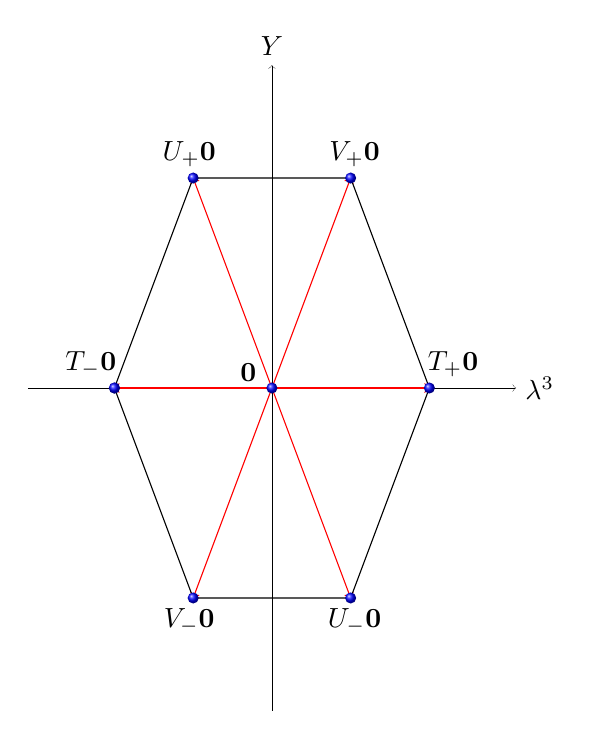
\begin{tikzpicture}
\draw[->,ultra thin] (-3.1,0)--(3.1,0) node[right]{$\lambda^3$};
\draw[->,ultra thin] (0,-4.1)--(0,4.1) node[above]{$Y$};
\draw[->, red] (0,0)--(-2, 0);
\draw[->, red] (0,0)--(2, 0);
\draw[->, red] (0,0)--(-1, 8/3);
\draw[->, red] (0,0)--(1, 8/3);
\draw[->, red] (0,0)--(1, -8/3);
\draw[->,red] (0,0)--(-1, -8/3);
  [anchor=mid west,
  mark size=+2pt, mark color=red,  ball color=green]
  \foreach \plm[count=\cnt] in {ball}
    \draw[mark options={fill=red}]
      plot[mark=\plm] coordinates {(-2, 0) (-1, 8/3) (1, 8/3) (2, 0) (1, -8/3) (-1, -8/3) (-2, 0)};
       [anchor=mid west,
  mark size=+2pt, mark color=red,  ball color=green]
  \foreach \plm[count=\cnt] in {ball}
    \draw[mark options={fill=red}]
      plot[mark=\plm] coordinates {(0, 0)};
	\node[] at (-2.3, 0.3) {$T_- \mathbf{0}$}; \node[] at (2.3, 0.3) {$T_+ \mathbf{0}$}; \node[] at (-1.05, 8/3 + 0.3) {$U_+ \mathbf{0}$};  \node[] at (1.05, 8/3 +0.3) {$V_+ \mathbf{0}$}; \node[] at (-1.05, -8/3-0.3) {$V_- \mathbf{0}$};  \node[] at (1.05, -8/3 -0.3) {$U_- \mathbf{0}$}; \node[] at (-0.3, 0.2) {$\mathbf{0}$};
\end{tikzpicture}
     
\end{figure}

The generators $\lambda^2$, $\lambda^5$ and $\lambda^7$, on the other hand, are essentially rotations with fixed axis $z$, $y$ and $x$ respectively. Therefore
\begin{equation*}\mathrm{Span}< \lambda^2, \, \lambda^5, \, \lambda^7 > \cong \mathrm{so}(3, \, \R), \end{equation*}
and the isomorphism is given by sending $\lambda^2$ to $\frac{1}{2} \tau^3$, $\lambda^5$ to $\frac{1}{2} \tau^2$ and $\lambda^7$ to $\frac{1}{2} \tau^1$. We notice that
\begin{equation*}\mathrm{tr}( \lambda^a \lambda^b ) = \frac{1}{2} \delta_{ab} \quad \text{and} \quad \mathrm{tr}( \tau^a \tau^b ) = 2 \delta_{ab}, \end{equation*}
which means that this is a minimal embedding of $\mathrm{so}(3, \, \R)$ into $\mathrm{su}(2, \, \C)$.

\section{Quark Model}

In physics an hadron is a subatomic particle (not elementary) that is subject to the strong nuclear force and is formed by quarks, sometimes associated to anti-quarks. Denote
\begin{equation*} |\, q\rangle = \begin{pmatrix} u \\ d \\ s \end{pmatrix} \quad \text{and} \quad |\, \bar{q}\rangle = \begin{pmatrix} \bar{u} \\ \bar{d} \\ \bar{s} \end{pmatrix} \end{equation*}
the quark and the anti-quark respectively. 

\paragraph{Baryons}\index{baryons} All known baryons are made of three valence quarks, so they are fermions, i.e., they have half-integer spin. In particular, we denote by
\begin{equation*} p, \, n, \, \Sigma^{-}, \, \Sigma^0, \, \Sigma^+, \, \Lambda, \, \Xi^0, \, \Xi^- \end{equation*}
the collection of the eight baryons of the form $| \, qqq \rangle$.

\paragraph{Mesons.}\index{mesons} Mesons are hadrons composed of a quark-antiquark pair. They are bosons, meaning they have integer spin, i.e., $0, 1$, or $-1$. In particular, we denote by
\begin{equation*} \pi^-, \, \pi^0, \, \pi^{+}, \, \kappa^+, \, \kappa^0, \, \bar{\kappa}^0, \, \kappa^-, \, \eta \end{equation*}
the collection of the eight mesons of the form $|\, q\bar{q} \rangle$.

\paragraph{Representation.} We can employ the weight diagrams introduced in the previous section to describe these octets in such a way to reveal some of their symmetries.

\begin{figure}[!htbp]
        \centering
        \mbox{%
\begin{minipage}{.45\textwidth}
\begin{tikzpicture}
\draw[->,ultra thin] (-2.6,0)--(2.6,0) node[right]{$\lambda^3$};
\draw[->,ultra thin] (0,-3.6)--(0,3.6) node[above]{$Y$};
  [anchor=mid west,
  mark size=+2pt, mark color=red,  ball color=green]
  \foreach \plm[count=\cnt] in {ball}
    \draw[mark options={fill=red}]
      plot[mark=\plm] coordinates {(-2, 0) (-1, 8/3) (1, 8/3) (2, 0) (1, -8/3) (-1, -8/3) (-2, 0)};
       [anchor=mid west,
  mark size=+2pt, mark color=red,  ball color=green]
  \foreach \plm[count=\cnt] in {ball}
    \draw[mark options={fill=red}]
      plot[mark=\plm] coordinates {(0, 0)};
	\node[] at (-2.3, 0.3) {$\pi^-$}; \node[] at (2.3, 0.3) {$\pi^+$}; \node[] at (-1.05, 8/3+0.3) {$\kappa^0$};  \node[] at (1.05, 8/3+0.3) {$\kappa^+$}; \node[] at (-1.05, -8/3-0.3) {$\kappa^-$};  \node[] at (1.05, -8/3-0.3) {$\bar{\kappa}^0$}; \node[] at (-0.3, 0.2) {$\pi^0$}; \node[] at (0.3, 0.2) {$\eta$};
\end{tikzpicture}
          \end{minipage}%
          \qquad
          \begin{minipage}{.45\textwidth}
     \begin{tikzpicture}
\draw[->,ultra thin] (-2.6,0)--(2.6,0) node[right]{$\lambda^3$};
\draw[->,ultra thin] (0,-3.6)--(0,3.6) node[above]{$Y$};
  [anchor=mid west,
  mark size=+2pt, mark color=red,  ball color=green]
  \foreach \plm[count=\cnt] in {ball}
    \draw[mark options={fill=red}]
      plot[mark=\plm] coordinates {(-2, 0) (-1, 8/3) (1, 8/3) (2, 0) (1, -8/3) (-1, -8/3) (-2, 0)};
       [anchor=mid west,
  mark size=+2pt, mark color=red,  ball color=green]
  \foreach \plm[count=\cnt] in {ball}
    \draw[mark options={fill=red}]
      plot[mark=\plm] coordinates {(0, 0)};
	\node[] at (-2.3, 0.3) {$\Sigma^-$}; \node[] at (2.3, 0.3) {$\Sigma^+$}; \node[] at (-1.05, 8/3+0.3) {$n$};  \node[] at (1.05, 8/3+0.3) {$p$}; \node[] at (-1.05, -8/3-0.3) {$\Xi^-$};  \node[] at (1.05, -8/3-0.3) {$\Xi^0$}; \node[] at (-0.3, 0.2) {$\Sigma^0$}; \node[] at (0.3, 0.2) {$\Lambda$};
\end{tikzpicture}
          \end{minipage}
    }
    \caption{On the left the mesons, and on the right the baryons.}
\end{figure}

The weight diagrams representation is coherent with the fact that, for example, the couple $(n, \, p)$ is an iso-duplet and $(\pi^-, \, \pi^0, \, \pi^+)$ is an iso-triplet, as we have already proved earlier. 

\newpage

The symmetry of $\mathrm{SU}(2, \, \C)$ is a "good symmetry" in nature, but the $\mathrm{SU}(3, \, \C)$ symmetry is broken by the masses since $m_u$ and $m_d$ are very near, while $m_s$ is comparable with $\Lambda_{QCD}$. More precisely, assuming $c = 1$, we have that
\begin{equation*}\begin{rcases} m_u \sim 5 \, \text{MeV} \\ m_d \sim 10 \, \text{MeV}  \end{rcases} \ll \Lambda_{QCD} \sim 200 \, \text{MeV} \quad \text{while $m_s \sim 200 \, \text{MeV}$}. \end{equation*}

\subsection{Young Tableaux}
\index{Young tableaux}

In mathematics, a Young tableau is a combinatorial object useful in representation theory. It provides a convenient way to describe the group representations of the symmetric and general linear groups $\mathfrak{S}_n$ and to study their properties.

We will not develop this topic here. The interested reader may consult \cite[Chapter 25.5]{hassani}. We only note that Young diagrams are in one-to-one correspondence with irreducible representations of the symmetric group over the complex numbers.

There is a nice way to introduce Young diagrams as a natural consequence of the symmetry properties of a system of $n$ particles interacting between themselves. We consider
\begin{equation*}\psi_{a_1}(1) \dots \psi_{a_n}(n), \end{equation*}
where $a_i \in \{1, \, \dots, \, p\}$ is, in a certain sense, the set of all properties.

The idea is to consider the symmetrization, anti-symmetrization and a mix of both of this expression with respect to the exchange of particles, and denote them via Young diagrams. For example, if $n = 2$ we have
\begin{equation*} \yng(2) = \frac{1}{\sqrt{2}} \left( \psi_{a_1}(1)\psi_{a_2}(2) + \psi_{a_2}(1)\psi_{a_1}(2) \right), \end{equation*}
and
\begin{equation*} \yng(1,1) = \frac{1}{\sqrt{2}} \left( \psi_{a_1}(1)\psi_{a_2}(2) - \psi_{a_2}(1)\psi_{a_1}(2) \right). \end{equation*}
Denote by $\psi_{1, \, 2}^S$ the symmetrization with respect to the indices $(1, \, 2)$, and denote by $\psi_{1, \, 2}^A$ the anti-symmetrization with respect to the indices $(1, \, 2)$. If $n = 3$ we have either a totally symmetric tensor, a totally antisymmetric tensor or a mix as follows:
\begin{equation*} \yng(3) = \frac{1}{\sqrt{3!}} \sum_{\sigma \in \mathfrak{S}_3} \psi_{a_1}(\sigma(1))\psi_{a_2}(\sigma(2)) \psi_{a_3}(\sigma(3))= \psi_{1, \, 2, \, 3}^S, \end{equation*}
\begin{equation*} \yng(1,1,1) = \frac{1}{\sqrt{3!}} \sum_{\sigma \in \mathfrak{S}_3}(-1)^{\mathrm{sgn}(\sigma)} \psi_{a_1}(\sigma(1))\psi_{a_2}(\sigma(2)) \psi_{a_3}(\sigma(3)) = \psi_{1, \, 2, \, 3}^A, \end{equation*}
and
\begin{equation*} \yng(2,1) = \sum_{\sigma \in \mathfrak{S}_2}(-1)^{\mathrm{sgn}(\sigma)} \psi_{1, \, \sigma(2)}^S \psi_{a_3}(\sigma(3)). \end{equation*}
The total symmetrization and anti-symmetrization can be computed explicitly for any value of $n$ and $p$ as follows:
\begin{equation*} \yng(3) \dots \yng(1) = \frac{1}{\sqrt{n!}} \sum_{\sigma \in \mathfrak{S}_n} \psi_{a_1}(\sigma(1))\psi_{a_2}(\sigma(2))\dots \psi_{a_n}(\sigma(n)), \end{equation*}
and
\begin{equation*} \begin{matrix} \yng(1,1,1) \\ \vdots \\ \yng(1) \end{matrix} = \begin{cases} \frac{1}{\sqrt{n!}} \sum_{\sigma \in \mathfrak{S}_n} (-1)^{\mathrm{sgn}(\sigma)} \psi_{a_1}(\sigma(1))\psi_{a_2}(\sigma(2))\dots \psi_{a_n}(\sigma(n)) & \text{if $n \leq p$},
\\[1em] 0 & \text{if $p > n$}. \end{cases} \end{equation*}

\paragraph{Special Unitary Group.} Let us consider neutrons of the form
\begin{equation*} | \, N \rangle := \begin{pmatrix} p \\ n \end{pmatrix} \end{equation*}
subject to the action of the special unitary group $\mathrm{SU}(2, \, \C)$. It is easy to check that
\begin{equation} \label{eq.9.1} \frac{p_1n_2 - n_1p_2}{\sqrt{2}} = \yng(1,1) \sim \underline{1}, \end{equation}
that is, the antisymmetric form corresponds to the singlet $\underline{1}$ as a consequence of the fact that the relation above is invariant under the action of $\mathrm{SU}(2, \, \C)$. Indeed, consider the vectors
\begin{equation*} \begin{pmatrix} p_1^\prime \\ n_1^\prime \end{pmatrix} = \begin{pmatrix} a & -b^\ast \\b & a^\ast \end{pmatrix} \begin{pmatrix} p_1 \\ n_1 \end{pmatrix} = \begin{pmatrix} a p_1 - b^\ast n_1 \\ b p_1 + a^\ast n_1\end{pmatrix}, \end{equation*}
and
\begin{equation*} \begin{pmatrix} p_2^\prime \\ n_2^\prime \end{pmatrix} = \begin{pmatrix} a & -b^\ast \\ b & a^\ast \end{pmatrix} \begin{pmatrix} p_2 \\ n_2 \end{pmatrix} = \begin{pmatrix} a p_2 - b^\ast n_2 \\ -b p_2 + a^\ast n_2\end{pmatrix}. \end{equation*}
A straightforward computation yields to
\begin{equation*}\begin{aligned} p_1^\prime n_2^\prime - n_1^\prime p_2^\prime & = (a p_1 - b^\ast n_1)(b p_2 + a^\ast n_2) - ( b p_1 + a^\ast n_1)(a p_2 - b^\ast n_2) =
\\[1em] & = - b b^\ast n_1 p_2 - a a^\ast n_1 p_2 + a a^\ast p_1 n_2 + b b^\ast p_1 n_2 =
\\[1em] & = p_1 n_2 - n_1 p_2, \end{aligned}\end{equation*}
and this proves the invariance under the action of $\mathrm{SU}(2, \, \C)$. The antisymmetric form corresponds to the so-called \textit{deuteron}, whose electric charge is one. In a similar way, one can prove that
\begin{equation*} \yng(2) \sim \underline{3}, \qquad \yng(3) \sim \underline{4}, \qquad \text{etc...} \end{equation*}
On the other hand, here $n$ is equal to $2$, and this means that the unique totally antisymmetric setting is the invariant one described above, that is,
\begin{equation*} \yng(1,1,1) = 0. \end{equation*}
In particular, a Young diagram for the group $\mathrm{SU}(2, \, \C)$ is equivalent to a totally symmetric one since
\begin{equation*} \yng(2,1) = \yng(1) \qquad \text{or} \qquad \yng(3,1) = \yng(2) \end{equation*}

There is a simple rule, that can be found in \cite[Chapter 25.5]{hassani}, that allows us to find the decomposition of a direct product of two representations.

In the following example, we show that what we have already proved for $\mathrm{SU}(3, \, \C)$ may be obtained via Young diagrams in a simple and coherent way. We shall now describe that rule, but we do not present any proof here.

\caution[b][green][Note]{The following result and the first application is taken, almost verbatim, from \cite[Chapter 25.5]{hassani}.}

\begin{theorem}[Young Rule \cite{hassani}] To find the components of Young frames in the product of two Young frames, draw one of the frames. In the other frame, assign the same symbol, say $a$, to all boxes in the first row, the same symbol $b$ to all the boxes in the second row, etc. Now attach the first row to the first frame, and enlarge in all possible ways subject to the restriction that no two $a$'s appear in the same column, and that the result graph be regular. Repeat with the $b$'s etc., making sure in each step that as we read from right to left and top to bottom no symbols counted fewer times than the symbol that came after it. The product is the sum of all the diagrams obtained in this way \end{theorem}

To illustrate this procedure, we shall compute the product $\underline{8} \otimes \underline{8}$ between representations of $\mathrm{SU}(3, \, \C)$. More precisely, consider the product
\begin{equation*} \Yvcentermath1 \yng(2,1) \otimes \young(11,2)  \end{equation*}
We now apply the first row $\young(11)$ to the frame on the left, and we obtain the following four Young diagrams:
\begin{equation*} \Yvcentermath1 \young(\empty\empty11,\empty) \qquad \young(\empty\empty1,\empty1) \qquad \young(\empty\empty1,\empty,1) \qquad \young(\empty\:,\empty1,1)   \end{equation*}
Now we apply the second row $\young(2)$ to each of these graphs separately.

\paragraph{First Diagram.} We cannot put a $2$ to the right of the $1$'s, because in that case, as we count from right to left, we would start with a $2$ without having counted any $1$'s. The allowed graphs obtain from the first diagram are thus given by
\begin{equation*} \Yvcentermath1 \young(\empty\empty11,\empty2) \qquad \young(\empty\empty11,\empty,2)   \end{equation*}

\paragraph{Second Diagram.} Applying the $\young(2)$ to the second graph yields to
\begin{equation*} \Yvcentermath1 \young(\empty\empty1,\empty12) \qquad \young(\empty\empty1,\empty1,2) \end{equation*}

\paragraph{Third Diagram.} Applying the $\young(2)$ to the third graph gives
\begin{equation*} \Yvcentermath1 \young(\empty\empty1,\empty2,1) \qquad \young(\empty\empty1,\empty,1,2) \end{equation*}

\paragraph{Fourth Diagram.} Applying the $\young(2)$ to the fourth graph yields to
\begin{equation*} \Yvcentermath1  \young(\empty\:,\empty1,12) \qquad  \young(\empty\:,\empty1,1,2) \end{equation*}

In particular, the entire process described above can be easily written in terms of frames as follows:
\begin{equation*} \Yvcentermath1 \begin{aligned} \yng(2,1) \otimes \yng(2,1) & = \yng(4,2) + \yng(4,1,1) + \yng(3,3) \: + \dots \\[1em] & \dots + 2 \: \yng(3,2,1) + \yng(3,1,1,1) + \yng(2,2,2) + \yng(2,2,1,1) \end{aligned} \end{equation*}
On the other hand, we are dealing with two representations of $\mathrm{SU}(3, \, \C)$, which means that the Young column of length $3$ is the singlet. The result is thus given by
\begin{equation*} \Yvcentermath1 \begin{aligned}\underline{8} \otimes \underline{8} & = \yng(4,2) + \yng(3) + \yng(3,3) \: + \dots \\[1em] & \dots + 2 \: \yng(2,1) + \yng(2,2,2) =
\\[1em] & = \underline{27} + \underline{10} + \underline{10}^\ast + \underline{8} + \underline{8} + \underline{1} \end{aligned} \end{equation*}
The fifth addendum and the seventh addendum are zero because $N = p = 3$, and therefore every column of length $4$ or more is automatically zero (as we already mentioned above).

\begin{example}The fundamental representation of $\mathrm{SU}(3, \, \C)$ is given by
\begin{equation*} \underline{3} \sim \yng(1) \end{equation*}
while its adjoint is given by
\begin{equation*} \underline{3}^\ast \sim \yng(1,1) \end{equation*}
The reader may check, as an exercise, that the following computations are correct and compare them with the results we already know.
\begin{equation*} \Yvcentermath1 \begin{aligned} & \underline{3} \otimes \underline{3} \sim  \yng(1) \otimes \yng(1) = \yng(2) + \yng(1,1)  \sim \underline{6} \oplus \underline{3}^\ast
\\[1em] & \underline{6} \otimes \underline{3} \sim \yng(2) \otimes \yng(1) =  \yng(3) + \yng(2,1) \sim \underline{10} \oplus \underline{8}
\\[1em] & \underline{6} \otimes \underline{6} \sim \yng(2) \otimes \yng(2) =  \yng(4) + \yng(3,1) + \yng(2,2)
\\[1em] &\underline{3} \otimes \underline{3}^\ast \sim \yng(1) \otimes \yng(1,1) = \yng(2,1) + \yng(1,1,1)
	 \sim \underline{8} \oplus \underline{1}
\\[1em] & \underline{3}^\ast \otimes \underline{3}^\ast \sim \yng(1,1) \otimes \yng(1,1) = \yng(1,1,1,1) + \yng(2,1,1) + \yng(2,2) \end{aligned}\end{equation*}

 \end{example}
 
We now want to generalize the relation \eqref{eq.9.1}, that is, in the special unitary group $\mathrm{SU}(2, \, \C)$ the totally antisymmetric form corresponds to the singlet $\underline{1}$.

More precisely, we shall prove that the Young diagram with $N$ rows and $1$ column is the singlet in $\mathrm{SU}(N, \, \C)$ for all $N \in \N$. First, notice that we have
\begin{equation*} \begin{matrix} \yng(1,1,1) \\ \vdots \\ \yng(1) \end{matrix} = \frac{1}{\sqrt{n!}} \sum_{\sigma \in \mathfrak{S}_n} (-1)^{\mathrm{sgn}(\sigma)} \psi_{a_1}(\sigma(1))\psi_{a_2}(\sigma(2))\dots \psi_{a_n}(\sigma(n)), \end{equation*}
where the $a_i$s takes value in the set $\{1, \, \dots, \, n\}$. Let $U \in \mathrm{SU}(N, \, \C)$ be an arbitrary unitary transformation, and consider
\begin{equation*}\psi_i^\prime = U \psi_i \implies (\psi_i^\prime)_j = U_{j, \, \ell} (\psi_i)_\ell, \end{equation*}
where $(\psi_i)_\ell$ denotes the $\ell$th component of the $i$th vector. It suffices to prove that
\begin{equation*}\sum_{\sigma \in \mathfrak{S}_n} (-1)^{\mathrm{sgn}(\sigma)} \psi_{1}(\sigma(1))\psi_{2}(\sigma(2))\dots \psi_{n}(\sigma(n)) = \sum_{\sigma \in \mathfrak{S}_n} (-1)^{\mathrm{sgn}(\sigma)} \psi_{1}^\prime(\sigma(1))\psi_{2}^\prime(\sigma(2))\dots \psi_{n}^\prime(\sigma(n)), \end{equation*}
where $\psi_{i}(\sigma(j))$ denotes the component $(\psi_i)_j$. A simple computation yields to
\begin{equation*}\begin{aligned} \sum_{\sigma \in \mathfrak{S}_n} (-1)^{\mathrm{sgn}(\sigma)} \psi_{1}^\prime(\sigma(1))\dots \psi_{n}^\prime(\sigma(n)) & = \sum_{\sigma \in \mathfrak{S}_n} (-1)^{\mathrm{sgn}(\sigma)} U_{\sigma(1), \, \ell} (\psi_1)_\ell \dots U_{\sigma(n), \, \ell} (\psi_{n})_\ell =
\\[1em] & = \epsilon^{\sigma(1) \dots \sigma(n)} U_{\sigma(1), \, \ell} (\psi_1)_\ell \dots U_{\sigma(n), \, \ell} (\psi_{n})_\ell =
\\[1em] & = \epsilon^{\sigma(1) \dots \sigma(n)}  \mathrm{det}(U)  (\psi_1)_{\sigma(1)} \dots  (\psi_{n})_{\sigma(n)} =
\\[1em] & = \sum_{\sigma \in \mathfrak{S}_n} (-1)^{\mathrm{sgn}(\sigma)} \psi_{1}(\sigma(1)) \dots \psi_{n}(\sigma(n)), \end{aligned}\end{equation*}
which is exactly what we wanted to prove.

\subsection{Adjoint Representation}

The Young frame of the adjoint representation of a given representation is extremely easy to find, especially when we are dealing with $\mathrm{SU}(N, \, \C)$.

Indeed, we know that the Young column of length $N$ corresponds to the singlet $\underline{1}$ in $\mathrm{SU}(N, \, \C)$, and therefore, given a representation $\mathscr{R}$ with a Young frame, we can find the Young frame of $\mathscr{R}^\ast$ as the "smallest" one that attached to the one of $\mathscr{R}$ gives a singlet.

\begin{example}The adjoint of the fundamental representation $\underline{3} \sim \yng(1)$ is given by $\underline{3}^\ast \sim \yng(1,1)$ since
\begin{equation*} \begin{matrix} \yng(1,1) \\ \updownarrow \\ \yng(1) \end{matrix} = \yng(1,1,1) \sim \underline{1}. \end{equation*}
The adjoint of the representation $\underline{6} \sim \yng(2)$ is given by the square, i.e.
\begin{equation*} \underline{6}^\ast \sim \yng(2,2) \end{equation*}
since
\begin{equation*} \begin{matrix} \yng(2) \\ \updownarrow \\ \yng(2,2) \end{matrix} = \yng(2,2,2) \sim \underline{1}. \end{equation*} \end{example}

\subsection{Multiplicity}

There is an easy way to find, given an arbitrary Young frame, the corresponding representation in $\mathrm{SU}(3)$. Indeed, if we consider the number $p_1$ of squares in the first row that have no other square attached below them, and the number $p_2$ of squares in the first row that have no other square attached below them, then
\begin{equation*} N_3 = \frac{1}{2} (p_1 + 1)(p_1 + p_2 + 2)(p_2 + 1) \end{equation*}
is the corresponding representation. For example, we have that
\begin{equation*} \yng(3,1) \sim \underline{15} \end{equation*}
because $p_1 = 2$ and $p_2 = 1$.

\subsection{Baryons, Resonances and Colors Model}

Recall that the known baryons are made of three valence quarks, so they are fermions, i.e., they have half-integer spin. In particular, we denote by
\begin{equation*} p, \, n, \, \Sigma^{-}, \, \Sigma^0, \, \Sigma^+, \, \Lambda, \, \Xi^0, \, \Xi^- \end{equation*}
the collection of the eight baryons of the form $| \, qqq \rangle$. Using Young diagrams we infer that
\begin{equation*} \Yvcentermath1 
    |\,qqq \rangle \sim  \yng(1) \otimes \yng(1) \otimes \yng(1) = \yng(3) + \yng(2,1) + \yng(2,1) + \yng(1,1,1)  \sim \underline{10} \oplus \underline{8} \oplus \underline{8} \oplus \underline{1},\end{equation*}
and therefore we would like to know something more specific about the composition of the decuplet. We will not give any details, as this topic will most likely be presented in a better way in a Quantum Physics course, but we simply recall some basic facts.

The four $\Delta$ baryons form a quartet in the weight diagram of $\underline{10}$, and they are given by $\Delta^{++}$ (constituent quarks: $| \,uuu\rangle$), $\Delta^+$ ($|\,uud\rangle$), $\Delta^0$ ($|\,udd\rangle$), and $\Delta^-$ ($|\,ddd\rangle$), which respectively carry an electric charge of $+2$, $+1$, $0$, and $-1$. They have spin and isospin $\frac{3}{2}$, and mass $\sim 1240 \, \text{$MeV$/$c^2$}$.
\newpage

\begin{figure}[!htbp]
        \centering
        \mbox{%
\begin{tikzpicture}
\draw[->,ultra thin] (-4.1,0)--(4.1,0) node[right]{$\lambda^3$};
\draw[->,ultra thin] (0,-7.1)--(0,4.1) node[above]{$Y$};
  [anchor=mid west,
  mark size=+2pt, mark color=red,  ball color=green]
  \foreach \plm[count=\cnt] in {ball}
    \draw[mark options={fill=red}]
      plot[mark=\plm] coordinates {(-1, 0) (-3/2,3) (-1/2, 3) (1/2, 3) (3/2, 3) (1, 0) (1/2, -3) (0, -6) (-1/2, -3) (-1, 0)};
       [anchor=mid west,
  mark size=+2pt, mark color=red,  ball color=green]
  \foreach \plm[count=\cnt] in {ball}
    \draw[mark options={fill=red}]
      plot[mark=\plm] coordinates {(0, 0)};
	\node[] at (-1.55, 3.3) {$\Delta^-$}; \node[] at (-1.5, 0.3) {$\Sigma^{\ast -}$}; \node[] at (1.5, 0.3) {$\Sigma^{\ast+}$}; \node[] at (-0.55, 3.3) {$\Delta^0$};  \node[] at (0.55, 3.3) {$\Delta^+$};  \node[] at (1.55, 3.3) {$\Delta^{++}$}; \node[] at (-0.85, -3.3) {$\Xi^{\ast-}$};  \node[] at (0.85, -3.3) {$\Xi^{\ast 0}$}; \node[] at (-0.3, 0.3) {$\Sigma^{ \ast 0}$}; \node[] at (0.4, -6.1) {$\Omega^-$}; 
\end{tikzpicture}
    }
    \caption{The decuplet of baryons. Note that the charge is constant on each diagonal and takes value in $\{-1, \, 0, \, 1, \, 2\}$.}
\end{figure}


The baryon $\Omega^-$ is given by $|\, sss \rangle$ and, as we will see in a few moments, this is one of the reasons why we need to introduce the notion of \textit{colors}. First, notice that
\begin{equation*} m_{\Omega^-} \sim 1650 \, \text{$MeV$/$c^2$}, \end{equation*}
which is way different from the energy of the $\Delta$ baryons since the symmetry in $\mathrm{SU}(3, \, \C)$ is broken by the introduction of the strange quark $s$, which brings a mass comparable to $\Lambda_{QCD}$, and this does not happen for $u$ and $d$.

Furthermore, the baryon $|\, sss \rangle$ is totally symmetric with respect to the space, and this is a direct contradiction with the Fermi-Dirac statistic, which asserts that it should be totally antisymmetric. 

\section{Fundamental Representation in $\mathrm{SU}(2, \, \C) \times \mathrm{U}(1, \, \C)$}

In this section, we want to decompose the irreducible representation $\underline{8}$ of $\mathrm{SU}(3, \, \C)$ in the product of irreducible representations of $\mathrm{SU}(2, \, \C) \times \mathrm{U}(1, \, \C)$. Recall that
\begin{equation*} Y = \frac{2}{\sqrt{3}} T^8 \quad \text{and} \quad \underline{3} \sim \yng(1) \sim \left(2, \, \frac{1}{3} \right) \oplus \underbracket{\left(1, \, - \frac{2}{3} \right)}_{\sim \: \young(3)}\end{equation*}
It follows that
\begin{equation*} \begin{aligned} \underline{8} & \sim \yng(2,1) = \young(\:3,\:) + \young(33,\empty) + \yng(2,1) + \young(\:\:,3) =
\\[1em] & = (\underline{1}, \, 0) +  (\underline{2}, \, -1) +  (\underline{2}, \, 1) +  (\underline{3}, \, 0). \end{aligned} \end{equation*}
since both ${\tiny \young(33,3)}$ and ${\tiny \young(3\:,\:)}$ are zero.